\chapter{\label{sec:dispmapanim} Evaluation of Displacement Mapped Models}

In chapter \ref{sec:dispmapcreation}, we presented a method of creating displacement maps for layered models, and for reconstructing a detailed surface from the displacement mapped representation. We begin this chapter by evaluating the quality of these reconstructions, proving that our method is capable of creating an accurate representation of a surface.

Displacement maps can also be easily edited to allow the detailed surface to be changed in a simple manner. In order to allow such editing using standard image tools, we must store the displacement map in a standard image format. The use of images for displacement map storage also has applications for compression of 3D mesh data. In this chapter, we will discuss each of these applications in turn, and in the process demonstrate the full capabilities of the displacement-mapped layered model architecture.

\section{\label{sec:dispmapanim:reconstructionresults}Reconstruction Quality}

To prove that our representation is valid, we will evaluate the quality of the reconstructed models, measuring how surface error is affected by the subdivision and rebuilding process. There are a number of possible sources of error in surface reconstruction:

\begin{itemize}
\item {\bf Subdivision Level}. The largest source of error will come from the level of subdivision that the model is reconstructed to. A coarse mesh simply cannot represent all of the detail in the dense surface, so error is inevitable. This error will reduce at higher subdivision levels.
\item {\bf Non-injectivity}. If the mapping from the detail layer to the control mesh is non-injective, as described in section \ref{sec:dispmapcreation:folding}, the displacement map cannot fully represent the entire detail layer, so some information will be lost.
\item {\bf Resolution}. The displacement map can only store one surface sample per pixel, so the larger the displacement map image, the more detail can be recovered in the rebuilt model. A small displacement map may also introduce pixel artifacts on the rebuilt surface, where multiple subdivided triangles have a displacement value from a single pixel.
\item {\bf Quantisation}. If the displacement map has been quantised for storage in an image format, only certain displacement values can be stored in the resulting map. Pixels with different values in the original map may have the same value in a quantised map. This will make the reconstructed surface less smooth, and may introduce a ``terraced'' effect in extreme cases.
\item {\bf Compression}. If the displacement image is compressed using a lossy algorithm, some fine details will be discarded during the process, again making the reconstruction from such a map less accurate.
\end{itemize}

We will evaluate each of these effects in turn.

\subsection{\label{sec:dispmapanim:reconstructionresults:metro}Metro}

In order to measure the accuracy of our method, we use the {\it Metro} tool developed by \citet{Cignoni98a} to measure the approximation error between the original and reconstructed surfaces. Metro measures the error between two polygonal surfaces, and calculates a number of overall statistics, including surface area, volume, and maximum and mean errors. 

We are particularly interested in the root mean squared (RMS) error, which will give us an overall indication of the accuracy of our displacement map reconstruction process. However, this value will depend on the scale of the model, so we normalise by the length of the diagonal of the bounding box of the mesh to give us a scale-invariant error metric.

\begin{figure}
\begin{center}
\begin{tabular}{cccc}
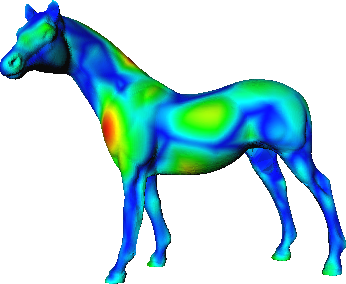
\includegraphics[width=3cm]{../images/horse_metro0} &
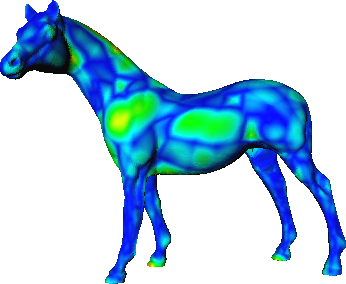
\includegraphics[width=3cm]{../images/horse_metro1} &
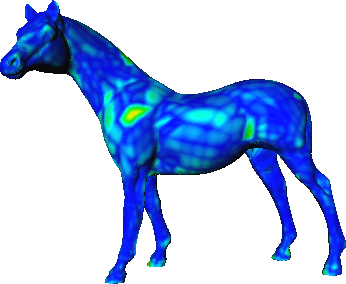
\includegraphics[width=3cm]{../images/horse_metro2} &
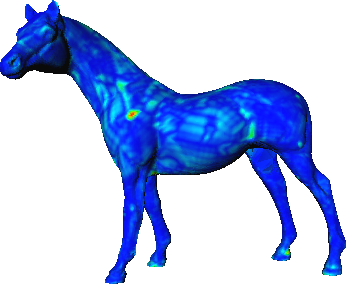
\includegraphics[width=3cm]{../images/horse_metro3} \\
{\it Level 0} & {\it Level 1} & {\it Level 2} & {\it Level 3}
\end{tabular}
\caption[Measuring Error with Metro]{\label{fig:measuremetro} Measuring Error with Metro. The surface colour shows shows the error between the original detail layer and the subdivided mesh. Blue areas have low error, while red areas have a high error value.}
\end{center}
\end{figure}

Metro can also create a graphical representation of the error across the surfaces, as a colour coding on the surface of the primary mesh. Figure \ref{fig:measuremetro} shows this error rendering shown on the Horse model. The model shown is the original detailed mesh, and the colour shows the difference between the reconstructed and original surfaces at various levels of subdivision. Red areas indicate large errors, while blue areas have a low error.

\subsection{\label{sec:dispmapanim:reconstruction:results:method}Method}

We have used Metro to analyse the error introduced by the process of reconstructing detailed meshes from our displacement map representations. In each case, a displacement mapped model is created as described in chapter \ref{sec:dispmapcreation}. The model is then subdivided uniformly a number of times. At each level of subdivision, the resulting model is compared to the original detailed mesh to give an indication of the quality of the reconstruction.

\subsection{\label{sec:dispmapanim:reconstruction:results:reconquality}Reconstruction Quality}

Our displacement map algorithm must provide an accurate reconstruction of the original model if it is to be useful. We will now measure the accuracy of reconstruction for the models shown in figure \ref{fig:models}. Reconstruction is performed using the uniform subdivision method, for up to six levels of subdivision. At each level, the normalised root mean squared surface error is measured using Metro. The error values for each model and level of subdivision are shown in table \ref{tbl:reconerror}, and illustrated in figure \ref{fig:reconerror}.

\begin{table}
\begin{center}
\begin{tabular}{c||cccc} 
Level & Cubehead & Monster & Horse & Bunny \\
\hline
0 & 7.8875\% & 2.7322\%  & 1.302\%   & 3.0029\% \\
1 & 3.0433\% & 1.5201\%  & 0.453\%   & 0.9588\% \\
2 & 1.5475\% & 0.8745\%  & 0.1634\%  & 0.4027\% \\
3 & 0.7839\% & 0.3562\%  & 0.06417\% & 0.1669\% \\
4 & 0.3812\% & 0.1647\%  & 0.0364\%  & 0.0868\% \\
5 & 0.2354\% & 0.1078\%  &         & \\
6 & 0.1869\% & 0.09063\% &         &
\end{tabular}
\caption[Reconstruction Error]{\label{tbl:reconerror} Reconstruction Error. Figures shown are the RMS surface error as a percentage of the length of the bounding box diagonal.}
\end{center}
\end{table}

\begin{figure}
\begin{center}
\begin{tabular}{cc} 
\includegraphics[width=7cm]{../graphs/dispmap_error} & 
\includegraphics[width=7cm]{../graphs/dispmap_error_log} \\
{\it(a)} & {\it(b)}
\end{tabular}
\caption[Reconstruction Error]{\label{fig:reconerror} Reconstruction Error. The graphs show how the normalised root mean squared surface error reduces with each subdivision step. (a) RMS shown on linear scale. (b) RMS shown on logarithmic scale.}
\end{center}
\end{figure}

As is to be expected, these figures show us that surface error decreases with each subdivision step, by a factor of between 2.5 and 3 at each step, depending on the model. Initial surface error values can tell us about the quality of the control model used to generate the map. The Cubehead model uses a stock model that is not based at all on the detail layer mesh, and as such has a higher initial surface error. Also, the ratio of control layer to detail layer polygon count is lower than in other models, meaning that more subdivision steps are required to obtain an accurate model of the surface. 

The Monster model uses an interactively-created control model, and its initial error is much lower as the control and detail layers are coincident at control layer vertices. The error is still generally high however, as the polygon count ratio is still low, roughly a fifth of the automatically-generated models. 

By virtue of having a large number of control layer triangles, and being generated directly from the detail layer, the automatically-generated Horse and Bunny models have low initial errors and require relatively few subdivision steps to closely approach the shape of the original detail layer. Errors are also lower for the automatically generated models as the displacement map is guaranteed to be injective, so no detail is lost in the generation process.

\subsection{\label{sec:dispmapanim:reconstruction:results:imagesize}Effect of Image Size}

We have also analysed the effect that the resolution of the displacement image has on the quality of the reconstruction results. This analysis was performed using the Monster mesh shown in figure \ref{fig:models}, but with displacement maps generated at resolutions of $256\times256$, $512\times512$, and $1024\times1024$ pixels. The results are shown in table \ref{tbl:imagesize} and illustrated in figure \ref{fig:imagesize}.

\begin{table}
\begin{center}
\begin{tabular}{c||ccc} 
Level & $256\times256$ & $512\times512$ & $1024\times1024$ \\
\hline
0 & 2.6502\% & 2.7249\% & 2.7322\% \\
1 & 1.4755\% & 1.515\% & 1.5201\% \\
2 & 0.866\% & 0.8777\% & 0.8745\% \\
3 & 0.3628\% & 0.3598\% & 0.3562\% \\
4 & 0.1917\% & 0.165\% & 0.1647\% \\
5 & 0.1439\% & 0.1132\% & 0.1078\% \\
6 & 0.1127\% & 0.09747\% & 0.09063\%
\end{tabular}
\caption[Effect of Image Size]{\label{tbl:imagesize} Effect of Image Size. Figures shown are the RMS surface error as a percentage of the length of the bounding box diagonal.}
\end{center}
\end{table}

\begin{figure}
\begin{center}
\includegraphics[width=7.5cm]{../graphs/imagesize}
\caption[Effect of Image Size]{\label{fig:imagesize} Effect of Image Size. All resolutions tested perform similarly until subdivision level 2, at which point they diverge, with lower resolution images giving larger surface error. }
\end{center}
\end{figure}

These results show that at low levels of subdivision image resolution makes little difference, while at higher levels, the effect smaller images have higher surface error. This is explained by the fact that a mesh reconstructed from a low-resolution displacement map will have many subdivided triangles which lie wholly within a single displacement map pixel. This leads to pixel artifacts becoming visible on the reconstructed mesh, giving a ``terraced'' appearance. This effect could be reduced, however, by performing a bilinear interpolation on displacement values when they are sampled from the image. Instead of using the closest pixel, all adjacent pixels would be taken into account to calculate an interpolated value for the displacement. This should reduce pixel artifacts, even on low-resolution displacement maps.

\section{\label{sec:dispmapanim:animation}Animating Displacement Mapped Models}

Animation of displacement mapped models is carried out in a very similar way to the animation of the standard layered models described in chapter \ref{sec:scandata:pointtosurface:reconstruction:animation}. The control layer model is animated to provide the general shape of the desired model. The subdivision algorithm in section \ref{sec:dispmapanim:reconstruction} is then applied to create the desired level of detail.

\subsection{\label{sec:dispmapanim:animation:results}Animation Results}

\begin{figure}
\begin{center}
\begin{tabular}{ccc}
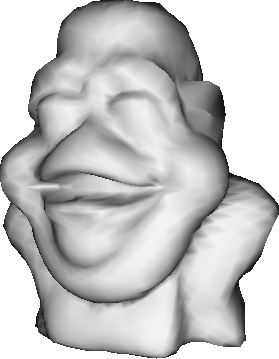
\includegraphics[width=3cm]{../images/dispanim_1} &
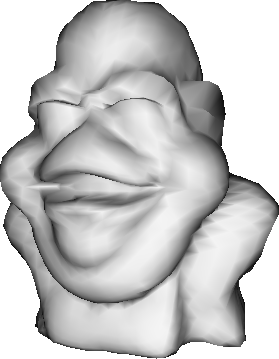
\includegraphics[width=3cm]{../images/dispanim_2} &
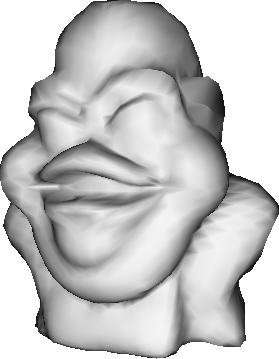
\includegraphics[width=3cm]{../images/dispanim_3} \\
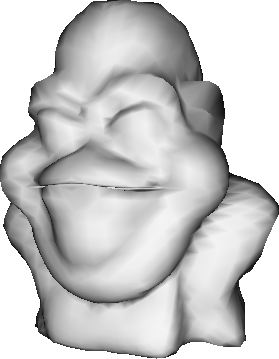
\includegraphics[width=3cm]{../images/dispanim_4} &
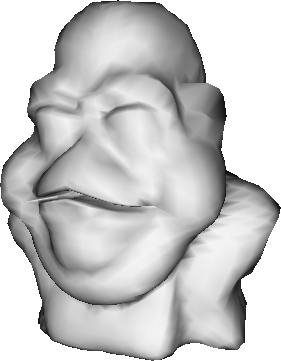
\includegraphics[width=3cm]{../images/dispanim_5} &
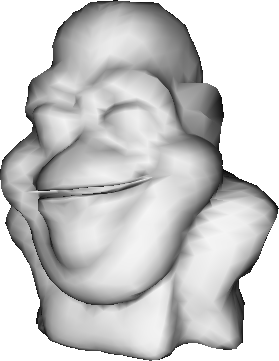
\includegraphics[width=3cm]{../images/dispanim_6} \\
& (a) &
\end{tabular}
\begin{tabular}{cc}
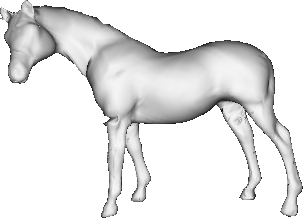
\includegraphics[width=4cm]{../images/horse_dispanim2} &
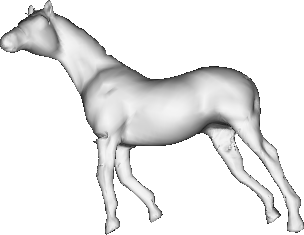
\includegraphics[width=4cm]{../images/horse_dispanim3} \\
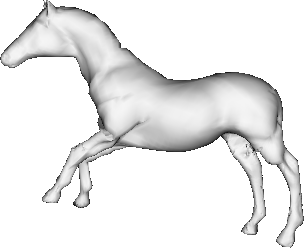
\includegraphics[width=4cm]{../images/horse_dispanim4} &
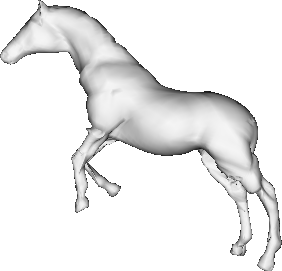
\includegraphics[width=4cm]{../images/horse_dispanim5} \\
\multicolumn{2}{c}{(b)}
\end{tabular}
\caption[Displacement Map Animation]{\label{fig:dispmapanim} Displacement Map Animation. Two models, rebuilt from displacement maps, performing the same animation sequences as in figure \ref{fig:detailanim}. (a) Facial animation of the Monster head, at four levels of uniform subdivision. (b) Horse animation, at three levels of uniform subdivision.}
\end{center}
\end{figure}

Figure \ref{fig:dispmapanim} shows a pair of animated models which have been reconstructed from displacement mapped representations. The animation sequences can be seen applied to the original dense surface data in figure \ref{fig:detailanim}. The animation has the same smoothness properties as the original detail layer animation, but has the advantage that the level of detail used can be specified by the user. This allows such animations to be performed in real time, using an appropriate level of reconstruction. As can be seen, only a small amount of subdivision is required to give a good approximation to the original model, and in applications where texture maps and other methods are be used to further improve the appearance of the subdivided models, this method of animation could be very valuable.

\subsection{\label{sec:dispmapanim:animation:distortion}Surface Distortion}

\begin{figure}
\begin{center}
\begin{tabular}{cc} 
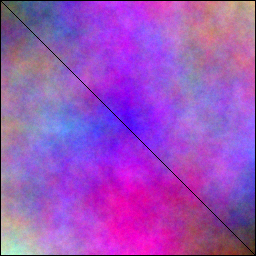
\includegraphics[width=5cm]{../images/texture_distort1} & 
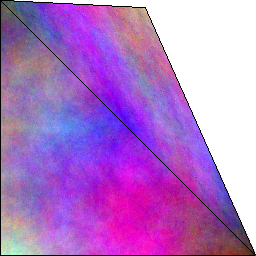
\includegraphics[width=5cm]{../images/texture_distort2} \\ 
{\it(a)} & {\it(b)}
\end{tabular}
\caption[Texture Distortion]{\label{fig:distortion} Texture Distortion. If adjacent triangles, shown in (a),  are not deformed in a similar fashion, texture and displacement maps can be distorted as seen in (b).}
\end{center}
\end{figure}
When the control layer surface is animated, the geometry of the mesh triangles changes. As the displacement map is attached to these triangles, this animates the reconstructed surface. However, under some circumstances, this change in geometry can become excessive and introduce distortion, as shown for a texture map in figure \ref{fig:distortion}. For instance, if a control layer triangle becomes degenerate under animation, the reconstruction of it's displacement map is likely to be incorrect. Distortion could also occur if one triangle changes shape much more than it's neighbours. If such distortion takes place, it will adversely affect the quality of the displacement map animation.

However, the skeletal animation method described in chapter \ref{sec:skeletalanim} should minimise unrealistic distortions and collapses of control layer triangles, as the surface deformation is spread evenly across multiple triangles during animation. This will prevent individual triangles from being distorted without the rest of the surface being affected, and instead will spread the distortion across the surface, reducing it's impact in any one area.

\section{\label{sec:dispmapanim:representation}Image Representations}

Once a displacement map has been generated, we need to store it on disk, for later reconstruction or transmission. We do this by storing the displacement map as we would a normal texture map, in a standard image file. We have investigated a number of different image file formats for storing displacement maps, as each format has advantages and disadvantages that will be discussed further in Section \ref{sec:dispmapanim:compression}.

However, if we are to use standard image formats, we must consider that these files cannot store displacement maps at their full level of detail. Displacement maps are created using a double-precision floating point number for each sample, normally corresponding to 64 bits per pixel. Images use $b\symbol{bits}$ bits to represent a pixel, where $b$ is relatively small (normally a maximum of 24), and also cannot store negative values. Therefore, the displacements that we have calculated for each pixel must be quantised appropriately.

In order to do this, we first find the maximum and minimum displacement values in the map, $[d_{max}, d_{min}]$, and then calculate the total range $r\symbol{range}$ of displacements.

\begin{equation}\label{eqn:range}
r = d_{max} - d_{min}
\end{equation}

We then use these values to calculate a quantised value $q_i\symbol{quantpixel}$ from each pixel $d_i$ in the displacement map.

\begin{equation}\label{eqn:quantise}
q_i = Int(\frac{d_i - d_{min}}r  (2^b-1))
\end{equation}

The quantised value is then stored in the appropriate pixel of the output image. $r$ and $d_{min}$ are stored in text comments in this file, where they can be read by the reconstruction software. 

Upon reconstruction of a displacement mapped model, we need to perform the inverse calculation, calculating a displacement value $d_i'$ from a quantised pixel $q_i$. 

\begin{equation} \label{eqn:recalcdistance}
d_i' = \frac{r q_i}{2^b-1} + d_{min}
\end{equation}

This quantisation process inevitably introduces a quantisation error $\varepsilon\symbol{quanterror}$ in the stored values, whose value is given by equation \ref{eqn:quanterror}.

\begin{equation}\label{eqn:quanterror}
\varepsilon = \frac{r}{2^{n+1}}
\end{equation}

This quantisation error can become visible in a reconstructed model under certain circumstances. If a displacement map has a large range $r$, but also contains features that vary over only a small part of this range, such small features will be lost if $\varepsilon$ is greater than the range covered by the feature. The number of bits $b$ used for quantisation must therefore be chosen carefully so that it is of the same order of magnitude as other errors, in order to preserve as much detail as possible.

\section{\label{sec:dispmapanim:editing}Mesh Editing}

In our displacement mapped models, the gross shape of the model is defined by the control layer, while the fine details are represented in the 2D displacement map. Since the mesh detail is encoded in such a simple 2D form, it makes it much easier to edit these details. Editing a complex mesh surface in 3D is a complicated task, but it is much simpler to edit a 2D image. If the displacement map is saved into a standard image format, it can be loaded into one of many common image editing programs. The displacement map can then be edited to add or remove detail, using paint or photo retouching tools. These changes will then be reflected in the reconstructed mesh.

For instance, a standard {\it lighten} photo retouching brush can be used to raise areas of the surface, while a {\it darken} brush can lower them. Performing image smoothing, either locally or globally, will smooth the surface, and various other image processing effects will produce a variety of interesting effects on the 3D surface. This property makes it easy for a 2D artist to be able to modify a 3D mesh without having to learn complex 3D editing tools. The mesh surface can be edited at the same time as a standard texture map, integrating the process of surface editing into one operation.

\begin{figure}
\begin{center}
\begin{tabular}{cc}
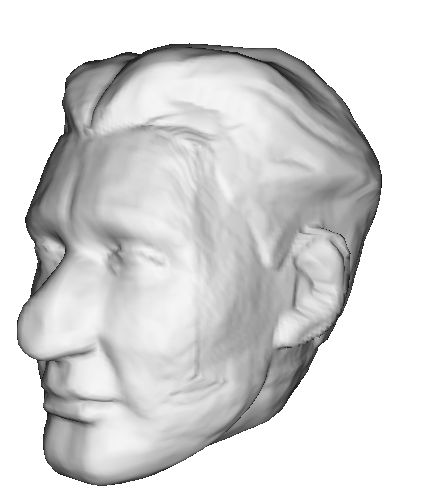
\includegraphics[width=6cm]{../images/editing_nose} &
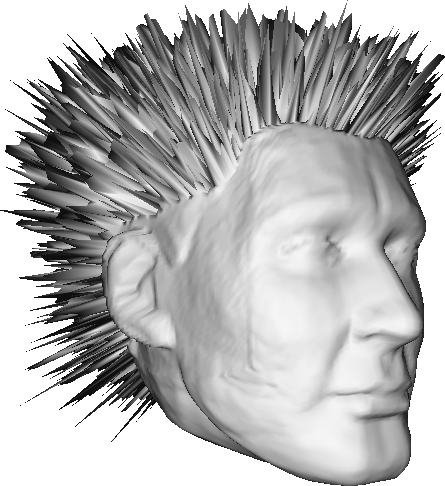
\includegraphics[width=6cm]{../images/editing_hair} \\
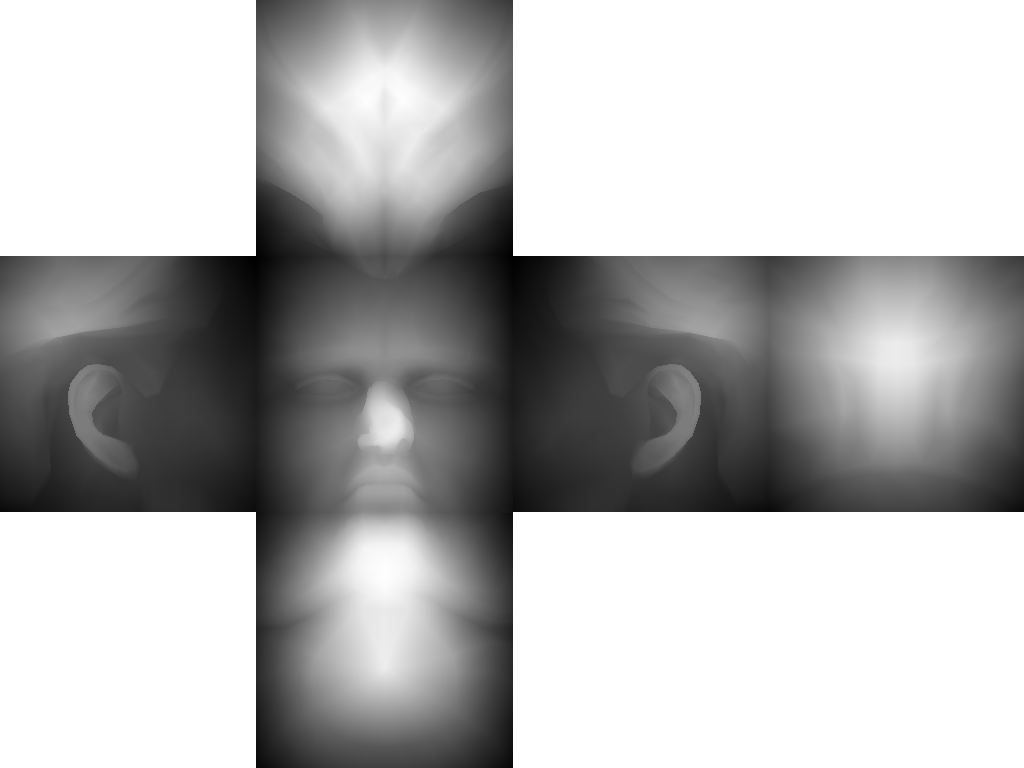
\includegraphics[width=6cm]{../images/editing_nose_map} &
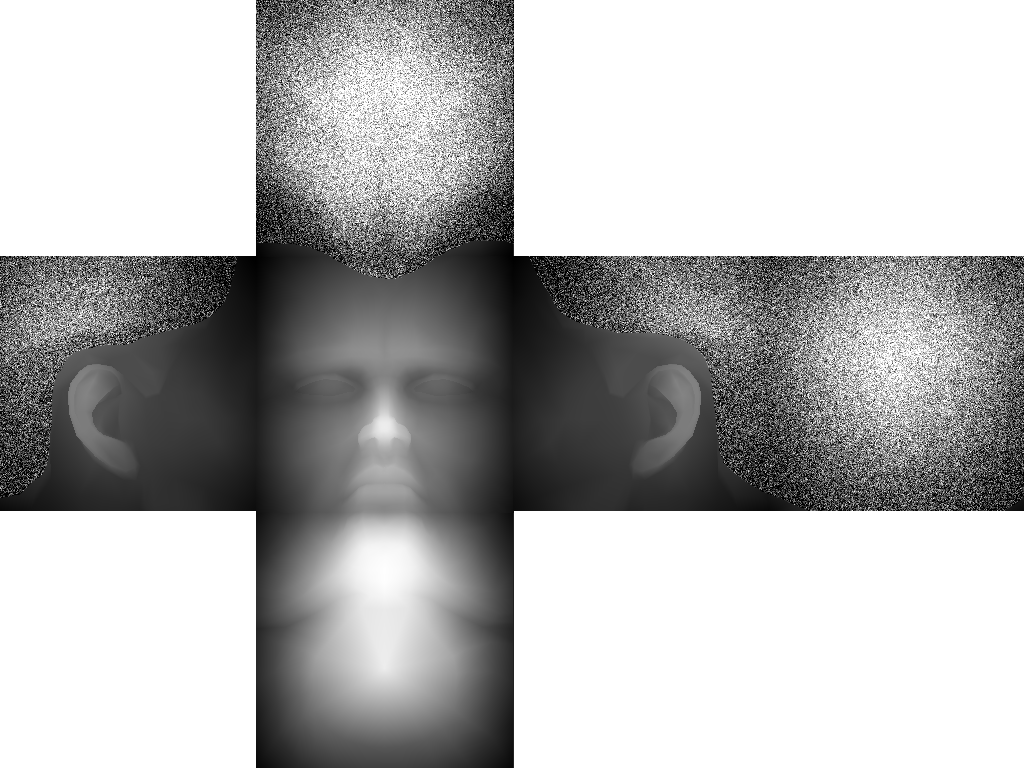
\includegraphics[width=6cm]{../images/editing_hair_map} \\
{\it (a)} & {\it (b)}
\end{tabular}
\caption[Mesh Editing Examples]{\label{fig:meshediting} Mesh Editing Examples. (a) Nose modification. (b) Random noise added to hair region. Surface noise is due to 8-bit quantisation of the edited images.}
\end{center}
\end{figure}

Figure \ref{fig:meshediting} shows a number of editing operations performed on the displacement mapped Cubehead model. These changes were performed using the freely-available GIMP image editing application.

\section{\label{sec:dispmapanim:compression}Displacement Compression}

Our displacement mapping approach is capable of representing each detail layer vertex as a single floating-point number, or a single byte in a quantised image format. This property implies that there is the potential to apply displacement map techniques to the compression of large polygon meshes, and also the progressive transmission thereof. Storing the data in an image format allows any part of the model to be refined as desired, but stores a large amount of extra data in order to facilitate this. However, image compression algorithms generally exploit spatial coherence in the image plane, so the data should be highly compressible as it is generally fairly coherent.

\subsection{\label{sec:dispmapanim:compression:images}Image Compression}

In the past, a large amount of research and development has been carried out in the field of still image compression, resulting in a selection of commonly-available compression algorithms and file formats \cite{Murray94}, including the widely used GIF, BMP, JPEG and PNG formats. The resulting algorithms can be applied to the compression of displacement mapped data.

We will investigate the compression capabilities of two of these major file formats - JPEG and PNG. Both of these formats are widely supported (a necessity if the resulting files are to be edited in standard tools), and both are capable of providing generally higher compression ratios than other competing formats. They also support a wide range of colour depths (i.e. number of bits per pixel stored) and multiple colour channels, which will be useful if a displacement map is to be stored in the same file as a standard texture map. We will first summarise the details of each compression method \cite{Miano99}.

\subsubsection{PNG Image Compression}

PNG \cite{Boutell97} uses a {\it lossless} compression scheme, meaning that no image information is lost in the compression and subsequent decompression process. It uses the {\it Deflate} compression algorithm, which is based on LZ77 compression and is also commonly used by the {\it gzip} file format.

\begin{figure}
\begin{center}
\begin{tabular}{ccccccc}

\includegraphics[width=1.5cm]{../images/adam7_1} &

\includegraphics[width=1.5cm]{../images/adam7_2} &
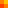
\includegraphics[width=1.5cm]{../images/adam7_3} &
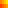
\includegraphics[width=1.5cm]{../images/adam7_4} &
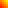
\includegraphics[width=1.5cm]{../images/adam7_5} &
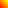
\includegraphics[width=1.5cm]{../images/adam7_6} &
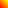
\includegraphics[width=1.5cm]{../images/adam7_7}
\end{tabular}
\caption[PNG Adam7 Interlacing]{\label{fig:adam7} PNG Adam7 Interlacing, showing the 7 levels for a single $8\times8$ block.}
\end{center}
\end{figure}

PNG also supports interlacing of image data using the {\it Adam7} method, which is used for progressive transmission of the image. The image is divided into $8\times8$ blocks, which are then divided into seven passes. The result of Adam7 interlacing on a single block is shown in figure \ref{fig:adam7}.

\subsubsection{JPEG Image Compression}

In contrast to PNG, the JPEG format is {\it lossy}. The JPEG standard defines a number of different compression schemes, but the most widely-used version involves dividing the image into $8\times8$ blocks, which are converted by a Discrete Cosine Transform (DCT) into a set of coefficient values. These coefficients are then quantised and Huffman coded before being stored in the JPEG file. The advantage of JPEG is that it can compress real-world images to a much greater degree than other formats, but it does this by discarding some image information. However, when creating a JPEG image, it is possible to select the quality of the final image, so it is possible for a user to manage the amount of data that is lost.  

\begin{figure}
\begin{center}
\begin{tabular}{ccccccc}
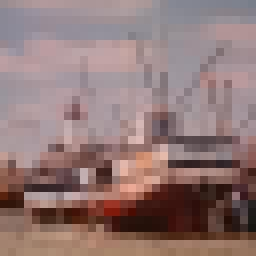
\includegraphics[width=1.5cm]{../images/jpeg_1} &
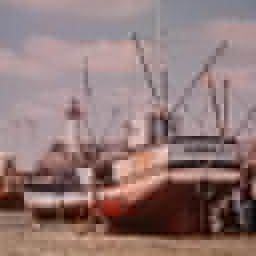
\includegraphics[width=1.5cm]{../images/jpeg_2} &
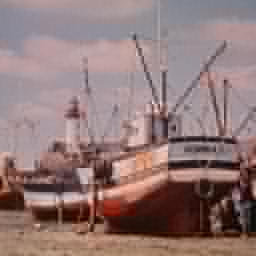
\includegraphics[width=1.5cm]{../images/jpeg_3} &
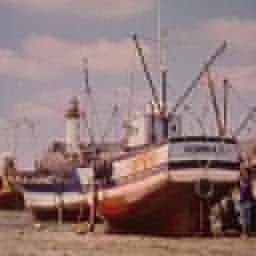
\includegraphics[width=1.5cm]{../images/jpeg_4} &
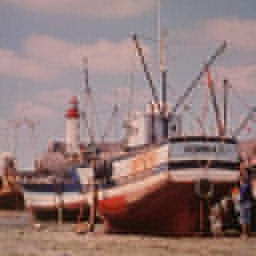
\includegraphics[width=1.5cm]{../images/jpeg_5} &
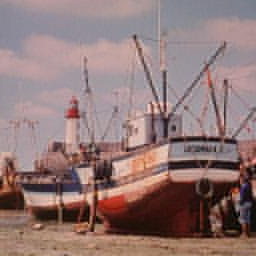
\includegraphics[width=1.5cm]{../images/jpeg_6} &
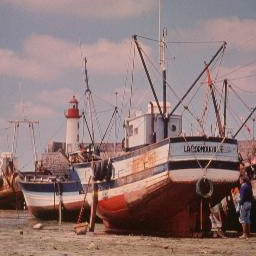
\includegraphics[width=1.5cm]{../images/jpeg_7}
\end{tabular}
\caption[Progressive JPEG]{\label{fig:progjpeg} Progressive JPEG, showing the quality of each level. Images taken from \cite{Rauschenbach}.}
\end{center}
\end{figure}

JPEG also supports progressive transmission by separating the image into a series of scans, each encoded at a higher quality than the last, examples of which are shown in figure \ref{fig:progjpeg}. JPEG also defines a lossless compression scheme; however, it is not in widespread use, and PNG provides higher compression ratios, so we will not consider lossless JPEG here.

\subsection{\label{sec:dispmapanim:compression:results}Results}

We have evaluated the effect of image compression algorithms in two ways. First, we evaluate the compression ratios for a number of meshes and sizes of displacement maps. This will give us an indication of the amount of compression that can be obtained. Secondly, we will investigate the effect of these image compression algorithms on the visual quality of the meshes.

\subsubsection{\label{sec:dispmapanim:compression:results:ratios}Compression Ratios}

We have generated a set of compressed displacement maps for the meshes shown in figure \ref{fig:models}. Displacement maps are generated at resolutions of $256\times256$, $512\times512$ and $1024\times1024$ pixels, which are quantised into an 8 bit per pixel representation. The resulting quantised images are then saved as PNG and JPEG with varying quality levels. We then calculate the compression ratio by comparing the resulting file sizes, including the size of the control mesh, to the size of the original mesh. All meshes are stored in gzipped OpenInventor format. The file sizes are shown in tables \ref{tbl:filesizes256}, \ref{tbl:filesizes512} and \ref{tbl:filesizes1024}.

\begin{table}
\begin{center}
\begin{tabular}{c||c|cccc|cccc|cccc}
 & & \multicolumn{4}{|c|}{$256\times256$} \\
Model & Original & PNG & JPG 95\% & JPG 75\% & JPG 50\% \\
\hline
Cubehead & 50160 & 
13197: 74\% & 5147: 90\% & 2385: 95\% & 1746: 97\% \\
Monster & 395926 & 
30954: 92\% & 13134: 97\% & 6371: 98\% & 4682: 99\% \\
Horse & 1009804 & 
64231: 94\% & 34320: 97\% & 24990: 98\% & 22708: 98\% \\
Bunny & 840545 & 
38743: 95\% & 27759: 97\% & 20196: 98\% & 18424: 98\% 
\end{tabular}
\caption[Compression Ratios for $256\times256$ Images.]{\label{tbl:filesizes256} Compression Ratios for $256\times256$ Images. All sizes are measured in bytes.}
\end{center}
\end{table}

\begin{table}
\begin{center}
\begin{tabular}{c||c|cccc|cccc|cccc}
 & & \multicolumn{4}{|c|}{$512\times512$} \\
Model & Original & PNG & JPG 95\% & JPG 75\% & JPG 50\% \\
\hline
Cubehead & 50160 & 
36596: 27\% & 14392: 71\% & 6004: 88\% & 4300: 91\% \\
Monster & 395926 & 
87235: 78\% & 34804: 91\% & 14709: 96\% & 10109: 97\% \\
Horse & 1009804 & 
144168: 86\% & 60993: 94\% & 36298: 96\% & 30151: 97\% \\
Bunny & 840545 & 
83073: 90\% & 48580: 94\% & 28291: 97\% & 23425: 97\% 
\end{tabular}
\caption[Compression Ratios for $512\times512$ Images.]{\label{tbl:filesizes512} Compression Ratios for $512\times512$ Images. All sizes are measured in bytes.}
\end{center}
\end{table}

\begin{table}
\begin{center}
\begin{tabular}{c||c|cccc|cccc|cccc}
 & & \multicolumn{4}{|c|}{$1024\times1024$} \\
Model & Original & PNG & JPG 95\% & JPG 75\% & JPG 50\% \\
\hline
Cubehead & 50160 & 
93434: -86\% & 40212: 20\% & 16783: 66\% & 12084: 76\% \\
Monster & 395926 & 
232188: 41\% & 92199: 77\% & 36080: 91\% & 24764: 94\% \\
Horse & 1009804 & 
324299: 68\% & 136062: 87\% & 66109: 93\% & 49834: 95\% \\
Bunny & 840545 & 
192102: 77\% & 108773: 87\% & 50470: 94\% & 38181: 95\% 
\end{tabular}
\caption[Compression Ratios for $1024\times1024$ Images.]{\label{tbl:filesizes1024} Compression Ratios for $1024\times1024$ Images. All sizes are measured in bytes.}
\end{center}
\end{table}

From these results we can see that displacement mapping, coupled with standard image compression algorithms, is indeed capable of compressing mesh data by a large amount compared to standard compression methods. Lossless PNG gives lower compression ratios than the lossy JPEG method, as is to be expected. This is mainly because JPEG exploits spatial coherence in the images better than PNG, and as our displacement maps vary in a generally smooth fashion, this is better suited to the JPEG compression scheme. 

\subsubsection{\label{sec:dispmapanim:compression:results:reconstr}Effect of Image Compression on Reconstruction}

In order to analyse the effect of these image compression algorithms on the quality of the reconstruction, we use the Monster model, and generate a $1024\times1024$ displacement map. A map of this size is used to minimise the effect of the image size on the results. The displacement map is then saved as an 8-bit quantised image file, again in both PNG and JPEG formats, and in the case of JPG, with various quality levels. The model is then reconstructed from these files, and the surface error measured with Metro at each subdivision level. The results are shown in table \ref{tbl:compression}, and illustrated in figure \ref{fig:compression}.

\begin{table}
\begin{center}
\begin{tabular}{c||c|cccc}
Level & Original & PNG & JPG 95\% & JPG 75\% & JPG 50\% \\
\hline
0 & 2.7322\% & 2.6128\% & 2.775\% & 2.768\% & 2.7345\% \\
1 & 1.5201\% & 1.5252\% & 1.5795\% & 1.5887\% & 1.5778\% \\
2 & 0.8745\% & 0.8917\% & 0.9081\% & 0.9075\% & 0.9149\% \\
3 & 0.3562\% & 0.3553\% & 0.3797\% & 0.3808\% & 0.3859\% \\
4 & 0.1647\% & 0.1677\% & 0.1775\% & 0.181\% & 0.1835\% \\
5 & 0.1078\% & 0.1111\% & 0.1203\% & 0.1234\% & 0.1265\% \\
6 & 0.09063\% & 0.0935\% & 0.1024\% & 0.1054\% & 0.11\%
\end{tabular}
\caption[Effect of Image Compression on Surface Error]{\label{tbl:compression} Effect of Image Compression on Surface Error. These figures were generated for the Monster model, using a $1024\times1024$ displacement map. The ``Original'' column represents the error obtained without translation to an image format.}
\end{center}
\end{table}

\begin{figure}
\begin{center}
\includegraphics[width=7.5cm]{../graphs/compression}
\caption[Effect of Image Compression on Surface Error]{\label{fig:compression} Effect of Image Compression on Surface Error. }
\end{center}
\end{figure}

As we can see from the table, at high levels of subdivision lossy JPEG compression gives us a higher surface error than lossless PNG, as is to be expected. We can also see that, as the quality of the JPEG compression is reduced, surface error again increases. As PNG compression does not lose any data, we can also conclude that the different between the Original and PNG error rates are solely due to the 8-bit quantisation required to store the displacement map as an image.

The figures in table \ref{tbl:compression} do not tell the full story, however. The differences in error rates are small, and based purely on these results it would seem that more compression is in general a good thing. However, the numbers only reflect the mean error across the entire surface. 

\begin{figure}
\begin{center}
\begin{tabular}{cc}
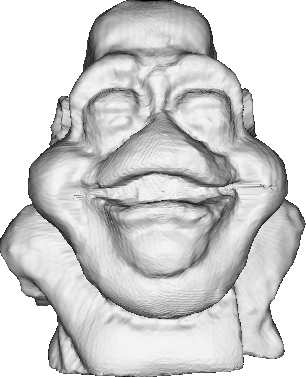
\includegraphics[width=6cm]{../images/compress_png} &
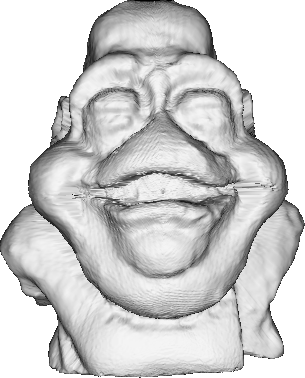
\includegraphics[width=6cm]{../images/compress_jpg95} \\
{\it (a)} & {\it (b)} \\
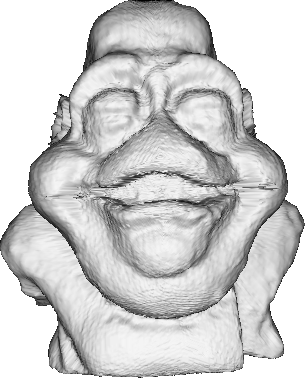
\includegraphics[width=6cm]{../images/compress_jpg75} &
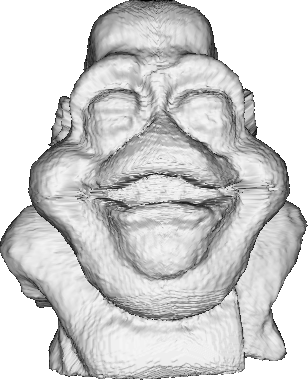
\includegraphics[width=6cm]{../images/compress_jpg50} \\
{\it (c)} & {\it (d)}
\end{tabular}
\caption[Visual Effect of Image Compression]{\label{fig:visual} Visual Effect of Image Compression. (a) PNG (b) JPEG 95\% (c) JPEG 75\% (d) JPEG 50\%. As the data loss in the compression process increases, visual artefacts increase.}
\end{center}
\end{figure}

If we look at the resulting reconstructions, shown in figure \ref{fig:visual}, we can see that for the lossy JPEG compression, a lower quality setting introduces noticeable artifacts. The subjective visual quality of the models is much worse than would be expected from the error measured by Metro. The appearance around texture seams is also much worse than for uncompressed images, caused by bleeding of pixel values due to the compression. Therefore, we can conclude that for this size of image, 75\% quality JPEG is probably the highest compression that we should use. 

The surface errors are caused by compression artifacts introduced into each $8\times8$ JPEG block. The lower the quality, the more error will occur inside a single block. The errors are also not smooth across block boundaries, causing discontinuities in the mesh surface. For a large displacement map, an $8\times8$ block will represent only a small area of the surface, so errors will be on a small scale. In smaller maps however, an $8\times8$ block will cover a much larger area of the surface, making these errors much more noticeable. This means that for smaller sizes of image, a higher quality setting will be required to give an visually acceptable surface when using lossy compression.

We can also draw some conclusions about the progressive mode of the various schemes, even without explicitly testing them. Progressive PNG effectively delivers a series of images at increasing resolution, meaning that the reconstruction quality will vary as shown in table \ref{tbl:imagesize} as the data is received. Initially, pixel artifacts would be visible on the surface, but these would disappear as more data becomes available. In the case of JPEG, the progressive mode is more akin to the use of multiple increasing quality levels. This would have the effect that initially the reconstructed surface would be noisy, as shown in figure \ref{fig:visual}d, but this noise would reduce as scans of higher quality were received. In both cases, if the subdivision level is tied to the amount of data received, it should be possible to progressively refine a model as more image data becomes available, without surface errors becoming noticeable.

\section{\label{sec:dispmapanim:conclusion}Conclusion}

In this chapter, we have presented a number of applications of the displacement mapped layered models introduced in chapter \ref{sec:dispmapcreation}. Reconstructed surfaces can be animated, driven by skeletal animation of the underlying control mesh, giving surface deformation that accurately reflect changes in the control mesh. Displacement maps also ease the process of editing mesh surfaces, as the map can be easily modified using standard 2D image editing tools, and changes will be reflected in the reconstructed surface. 

It is also possible to apply image compression techniques to the displacement maps, yielding useful levels of surface compression, and providing benefits for progressive transmission. Errors are introduced into the reconstructed meshes from various sources in the displacement mapping process, but by ensuring that one form of error does not dominate over the others, it should be possible to use displacement maps to easily create realistic images and animations based on densely scanned surface data.
